\section{The builder mechanism}

\subsection{Overview of the builder package \texttt{it.unibo.kaktor.builders}}

In addition to the transient model, we want to provide a sort of \textit{standard mechanism} that must be reliable and reusable to create the transient entities.

So, we decided to use the \href{https://en.wikipedia.org/wiki/Builder_pattern}{builder pattern}.

\begin{figure}[h]
	\centering
	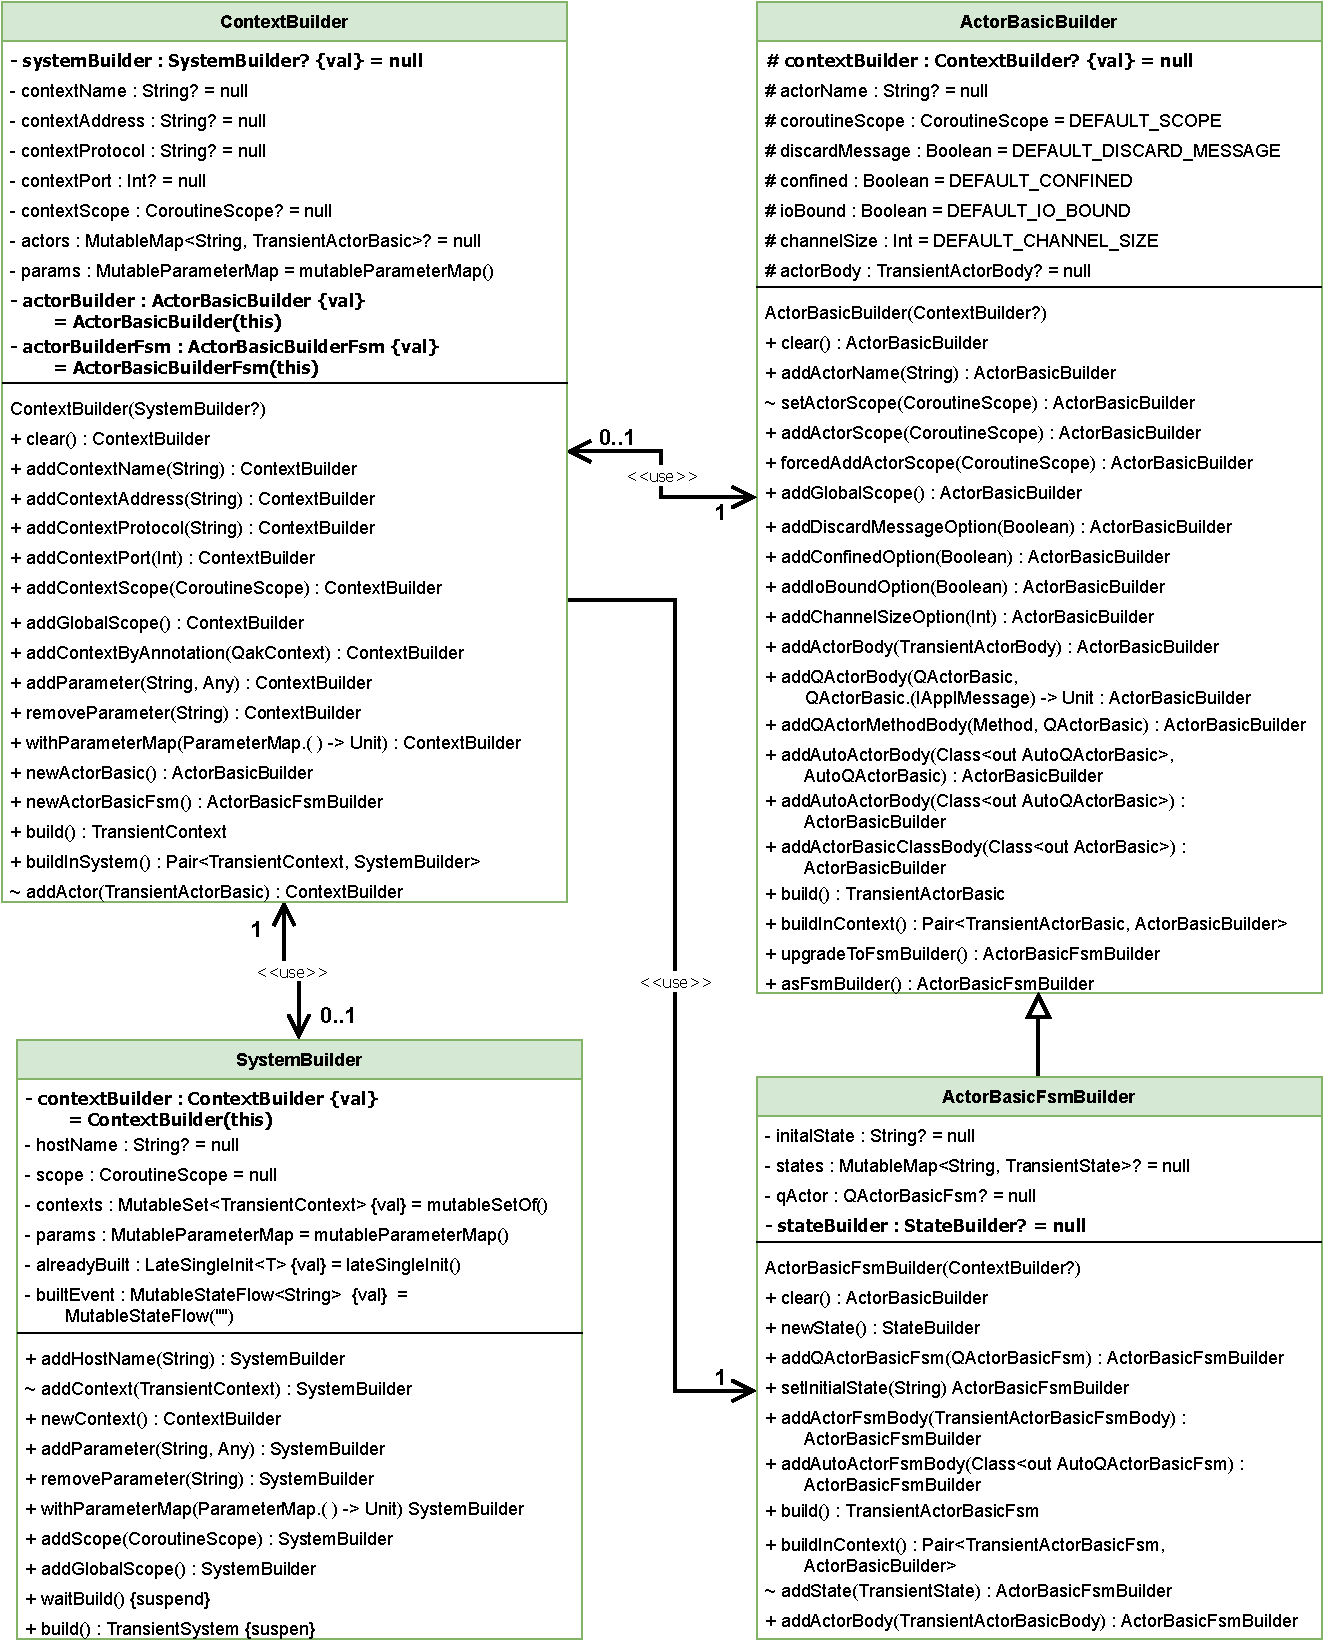
\includegraphics[width=0.92\textwidth]{img/[UML]it.unibo.kaktor.builders_actorb_contextb_systemb}
	\caption{UML diagram for the Transient Model of the actor body}
	\label{fig::builders_actorb_contextb_systemb}
\end{figure}

The figure \ref{fig::builders_actorb_contextb_systemb} shows the main builder components for the transient system. They are:
\begin{itemize}
	\item 	\underline{\textbf{\texttt{ActorBasicBuilder}}}:\\
	This component let to create a \texttt{TransientActorBasic} using the builder pattern. It is easy possible to set the actor body by calling the \verb*|addActorBoby(TransientActorBody)| method. There are others additional methods that can be used to quickly add  more complex body that the normal lambda body (the classes not already explained of the transient body model).
	
	\item 	\underline{\textbf{\texttt{ActorBasiFsmcBuilder}}}:\\
	This component let to create a \texttt{TransientActorBasicFsm} using the builder pattern. This class extends the \texttt{ActorBasicBuilder} then add others additional method to its in order to create a finite state machine actor. It is easy possible to add a state to the actor that is building by calling \verb*|newState()| method that returns a \texttt{StateBuilder} for the new state.
	
	\item 	\underline{\textbf{\texttt{ContextBuilder}}}:\\
	This component let to create a \texttt{TransientContext}. It is easy possible to add an actor to the context that is building by calling \verb*|newActorBasic()| or \verb*|newActorBasicFsm()| methods that return a builder for the new actor.
	
	\item 	\underline{\textbf{\texttt{SystemBuilder}}}:\\
	This component let to create a \texttt{TransientSystem}. It is easy possible to add a context to the system that is building by calling \verb*|newContext()| method that returns a \texttt{ContextBuilder}. When the creation of the transient system is completed so it is needed to invoke the \verb*|buil()| method that returns the \texttt{TransientSystem}. Notice that \textbf{a \texttt{SystemBuilder} cannot be reused then once the system is created it not possible to clear the builder and start again the creation}. In addition to this, after the build method invocation, there are no possibilities to add other contexts or to build again.
\end{itemize}

In addition to all things we have just explained, the builders can throw a \texttt{BuildException} if something goes wrong or if the developer has not passed all the needed information to it before invoking \verb*|build()|, for example if the developer invoke it without calling the \verb*|addActorName(String)| before.

\begin{figure}[h]
	\centering
	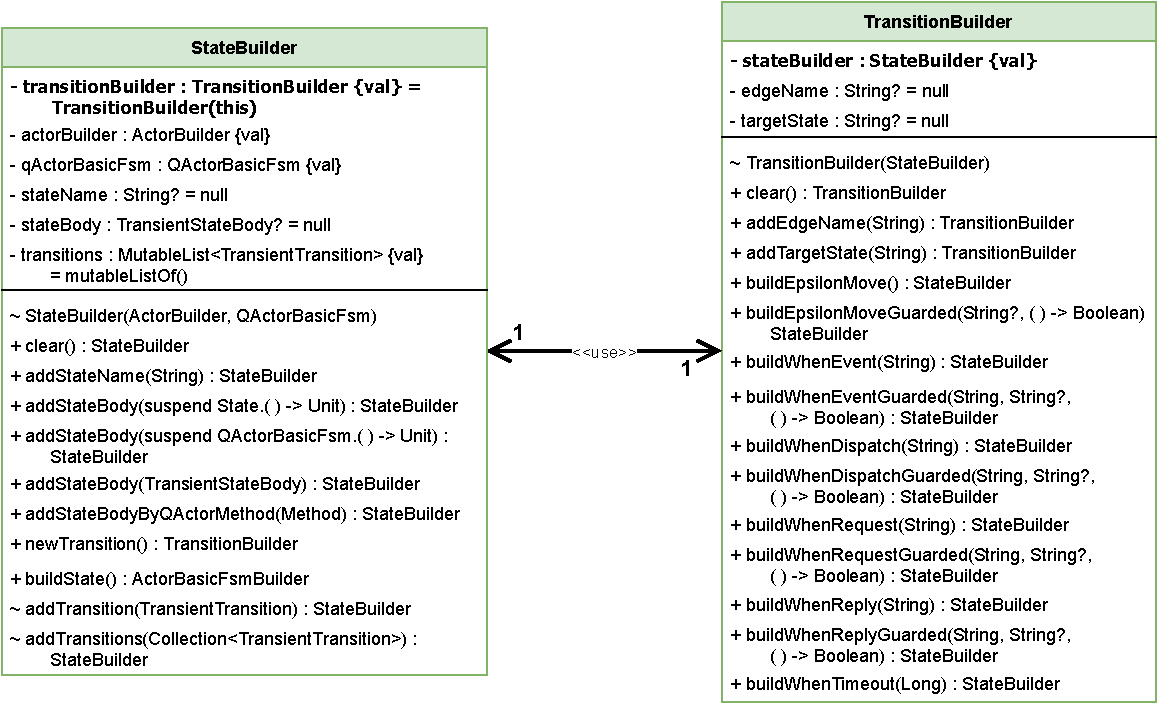
\includegraphics[width=\textwidth]{img/[UML]it.unibo.kaktor.builders_stateb_transitionb}
	\caption{UML diagram for the Transient Model of the actor body}
	\label{fig::builders_stateb_transitionb}
\end{figure}
As anticipated, for finite state machine actors we also provide some additional builders shown in the figure \ref{fig::builders_stateb_transitionb}:

\begin{itemize}
	\item 	\underline{\textbf{\texttt{StateBuilder}}}:\\
	The component for building states. If we have an \texttt{ActorBasicFsmBuilder} we can call the \verb*|newState()| method that returns an instance of the \texttt{StateBuilder} class that can be used to add states. When all of the states are added then it is possible to invoke the \texttt{buildState()} method that return the original actor builder. \textbf{Notice that it not possible to create a \texttt{StateBuilder} because it can only be obtained from an actor builder}.
	
	\item 	\underline{\textbf{\texttt{StateBuilder}}}:\\
	The component for building transitions. It can be obtained using the \verb*|newTransition()| method of the \texttt{StateBuilder} class with the same mechanism by which the state builder can be obtained from the actor builder. In addition, this component has more than one \texttt{build} method for each type of transition supported by the infrastructure.
\end{itemize}

\subsection{The wrappers}

As we have already said, the transient entities of the model are only a \textbf{passive description} of the system that will have to run. So this description must be transformed into the \textbf{executable units} that are present in the \texttt{QA} infrastructure: \texttt{ActorBasic} and \texttt{ActorBasicFsm}.

\begin{figure}[h]
	\centering
	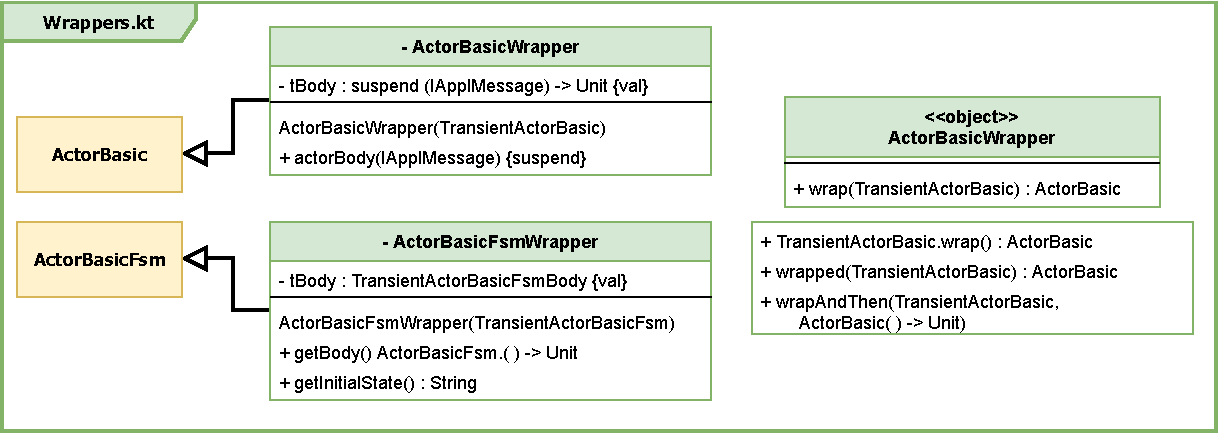
\includegraphics[width=\textwidth]{img/[UML]it.unibo.kaktor.builders_wrapper}
	\caption{UML diagram for the Transient Model of the actor body}
	\label{fig::builders_wrapper}
\end{figure}

The \texttt{Wrappers.kt} file contains the classes to \textbf{wrap} the \texttt{TransientActorBasic} and the \texttt{TransientActorBasicFsm} entities into the active entities of the \texttt{QA-System}.
This file also contains some extensions method for the \texttt{TransientActorBasic} class to quickly wrap it into an \texttt{ActorBasic} instance.

For the details about wrappers and their work, please see the source code.